\documentclass[../main/thesis.tex]{subfiles}

\graphicspath{{/home/arefk/uio/MScThesis_AreKvanum2022_SeaIceML/thesis/datasets/figures/}}

\begin{document}
\section{Datasets}
[Training and validating a deep learning system requires data, which can be categorized in two distinct groups. The first group is the data known by the system, which is used during training to increase or validate model performance. Due to developing the model in such a way that it performs well against its validation data, external data is needed to validate the generalizability of the model. I.e., how well does the model perform with unknown data, which is assumed drawn from the same distribution as the data used during training. It is standard practice to arbitrarily split by a given fraction into the three datasets (training, validation, tasting), as outlined above. However, due to the variable seasonal dependency of meteorological data, a naive split of the data could result in seasonally unbalanced datasets. As such, the datasets constructed for the purpose of this thesis are each covering at least a full year. Thus, no dataset is assumed to be skewed in the direction of any season.] \todo{Dette passer bedre inn i en train-test-split \textbf{model development}} 

To facilitate the development and verification of the developed deep learning system, several datasets covering observations and forecasting systems have been chosen. The following section will perform a rundown of the satellite products as well as physical models used. Table \ref{tab:data_overview} presents the different products used for this thesis, and whether the product is used to train or verify the model.

\begin{table}[]
    \caption{\label{tab:data_overview}Rundown of the products used and their applications. The dashed line separates observational products (above) from forecast products (below)}
    \centering
    \setlength{\arrayrulewidth}{0.5mm}
    \renewcommand{\arraystretch}{1.3}
    \begin{tabular}{llll}
    \hline
    Product             & Variables           & Training & Verification \\
    \hline
    Ice charts          & SIC                 & Yes      & Yes          \\
    OSI-SAF SSMIS       & SIC trend           & Yes      & Yes          \\
    OSI-SAF CDR         & Ice edge length     & No       & Yes          \\
    AMSR2               & SIC                 & No       & Yes          \\
    \hdashline
    AROME-Arctic        & T2M, X-wind, Y-wind & Yes      & No           \\
    NeXtSIM             & SIC                 & No       & Yes          \\
    Barents-2.5         & SIC                 & No       & Yes          \\
    \hline         
    \end{tabular}
\end{table}


\subsection{Region}
The region chosen as study area is a combination of the Greenland and Barents sea, and is a intersection of the domain covered by the Ice Charts \cite{Dinessen2020} with the domain covered by AROME Arctic \cite{Mueller2017} as shown in Figure (\ref{fig:studyarea-sketch}). The domain retained the spatial resolution of the Ice Charts and the projection of AROME Arctic, hence the domain is on a 1km equidistant Lambert conformal conic grid with 1972 grid-points in each direction. Furthermore, the southern and eastern extent of AROME Arctic was reduced to a square domain due to restrictions to the input data shape set by the deep learning architecture. It was deliberately chosen to reduce the extent in those directions, to limit the amount of sea ice lost and to still cover operationally important areas such as Svalbard. 

\begin{figure}
    \centering
    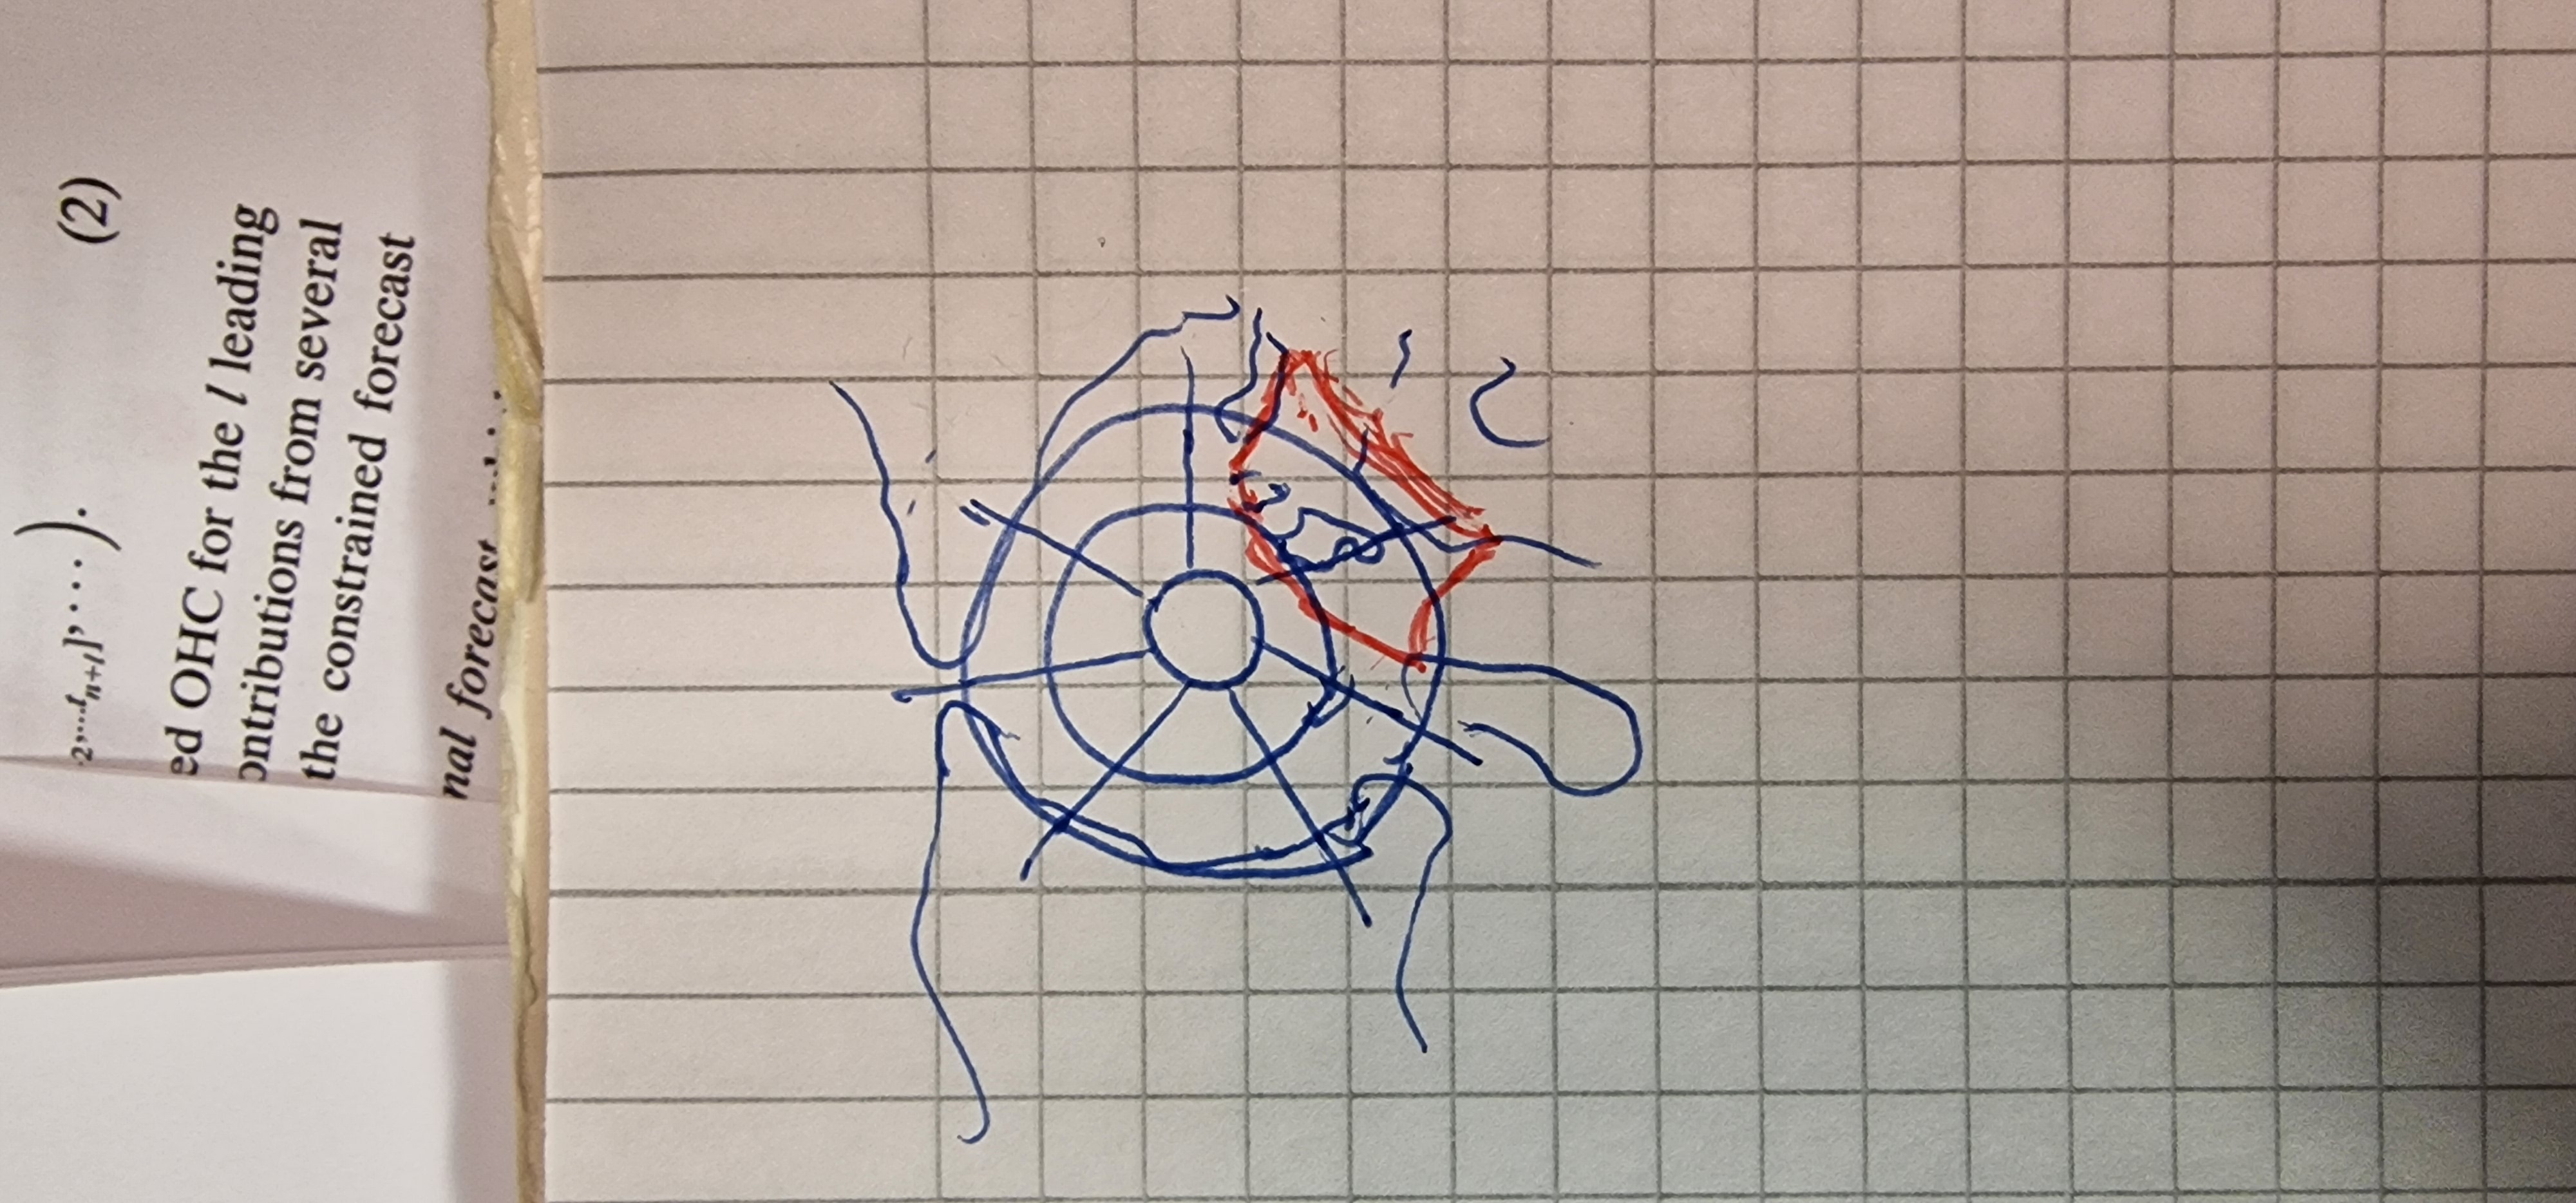
\includegraphics[width = .5\textwidth, angle = -90, trim = {40cm 0 50cm 0}, clip]{studyarea_sketch}
    \caption{\label{fig:studyarea-sketch}Sketch showing where the study-area is located from a pan arctic perspective}
\end{figure}




% The aim of this section is to perform a rundown of the different datasets used for the purpose of this thesis. This includes both internal datasets, in the sense that they are used for training the deep learning system, but also external datasets as in datasets only used for validating model performance. The term \textit{dataset} will for the scope of this thesis refer to a sequence of spatio-temporal structured arrays containing gridded values, and serves as a catch-all for model outputs and satellite products.

\subsection{Observations}

\subsubsection{Sea Ice Charts}

\begin{figure}
    \missingfigure{Få inn en figur som viser månedlig SIC fordeling fra Ice Chartsene, gjerne over en ti års periode. Som i Grigoryev2022}
\end{figure}

\begin{figure}
    \missingfigure{Få inn en figur som viser autocorrelation for IceChartsa gitt en viss periode.}
\end{figure}

The Sea Ice charts is an operational Sea Ice Concentration product provided by MET Norway. The product is manually drawn by a Sea Ice Specialist, and is distributed every workday at 15:00 UTC. The Sea Ice specialist assesses available SAR data from Sentinel 1 and Radarsat 2. However, due to the spatial variability in daily SAR coverage, visual, infrared and low resolution passive microwave observations are supplied to achieve a consistent spatial coverage \cite{MOI2015}. The Sea Ice charts are drawn in an ArcGIS production environment, and is as such intrinsically not projected onto a defined grid. Yet, the operational product available for download on \href{https://resources.marine.copernicus.eu/product-detail/SEAICE_ARC_SEAICE_L4_NRT_OBSERVATIONS_011_002/INFORMATION}{Copernicus} is provided as mean values on a 1km grid.

From the description of the Sea Ice charts given above, it is worth addressing the spatial inconsistency following the projection onto a uniformly sized grid. As the Sea Ice specialist draws polygons based on data from different satellite sources with a wide range of spatial resolution (80m from SAR, 1000m from visible / infrared and even lower resolution for passive microwave), the underlying uncertainty and detailed structures in the Sea Ice chart varies \cite{MOI2015}. Furthermore, I was made aware by one of the Sea Ice Analysts that time constraints also limits the hours different sections of the Ice chart is alloted. Moreover, the Sea Ice charts is an operational product aimed at end users in industries such as fishing, tourism, shipping or other maritime operations. This influences the decision-making when creating the final operational product. \todo{ask Trond on email}. As a consequence, the Sea Ice analyst spends approximately half of the total time draw polygons around the Svalbard archipelago. 

In conclusion, concerning the limited resources available both with regards to data availability as well as total hours available, the Sea Ice charts represents a dataset with a spatial uncertainty that is non-uniform across a single sample, and that changes in time. In spite of that, the involvement of a Sea Ice specialist which manually assures each Sea Ice charts, the temporal consistency as well as their high resolution has led us to believe that the Sea Ice charts is the overall best Sea Ice Concentration product available for the current study region.

\begin{figure}
    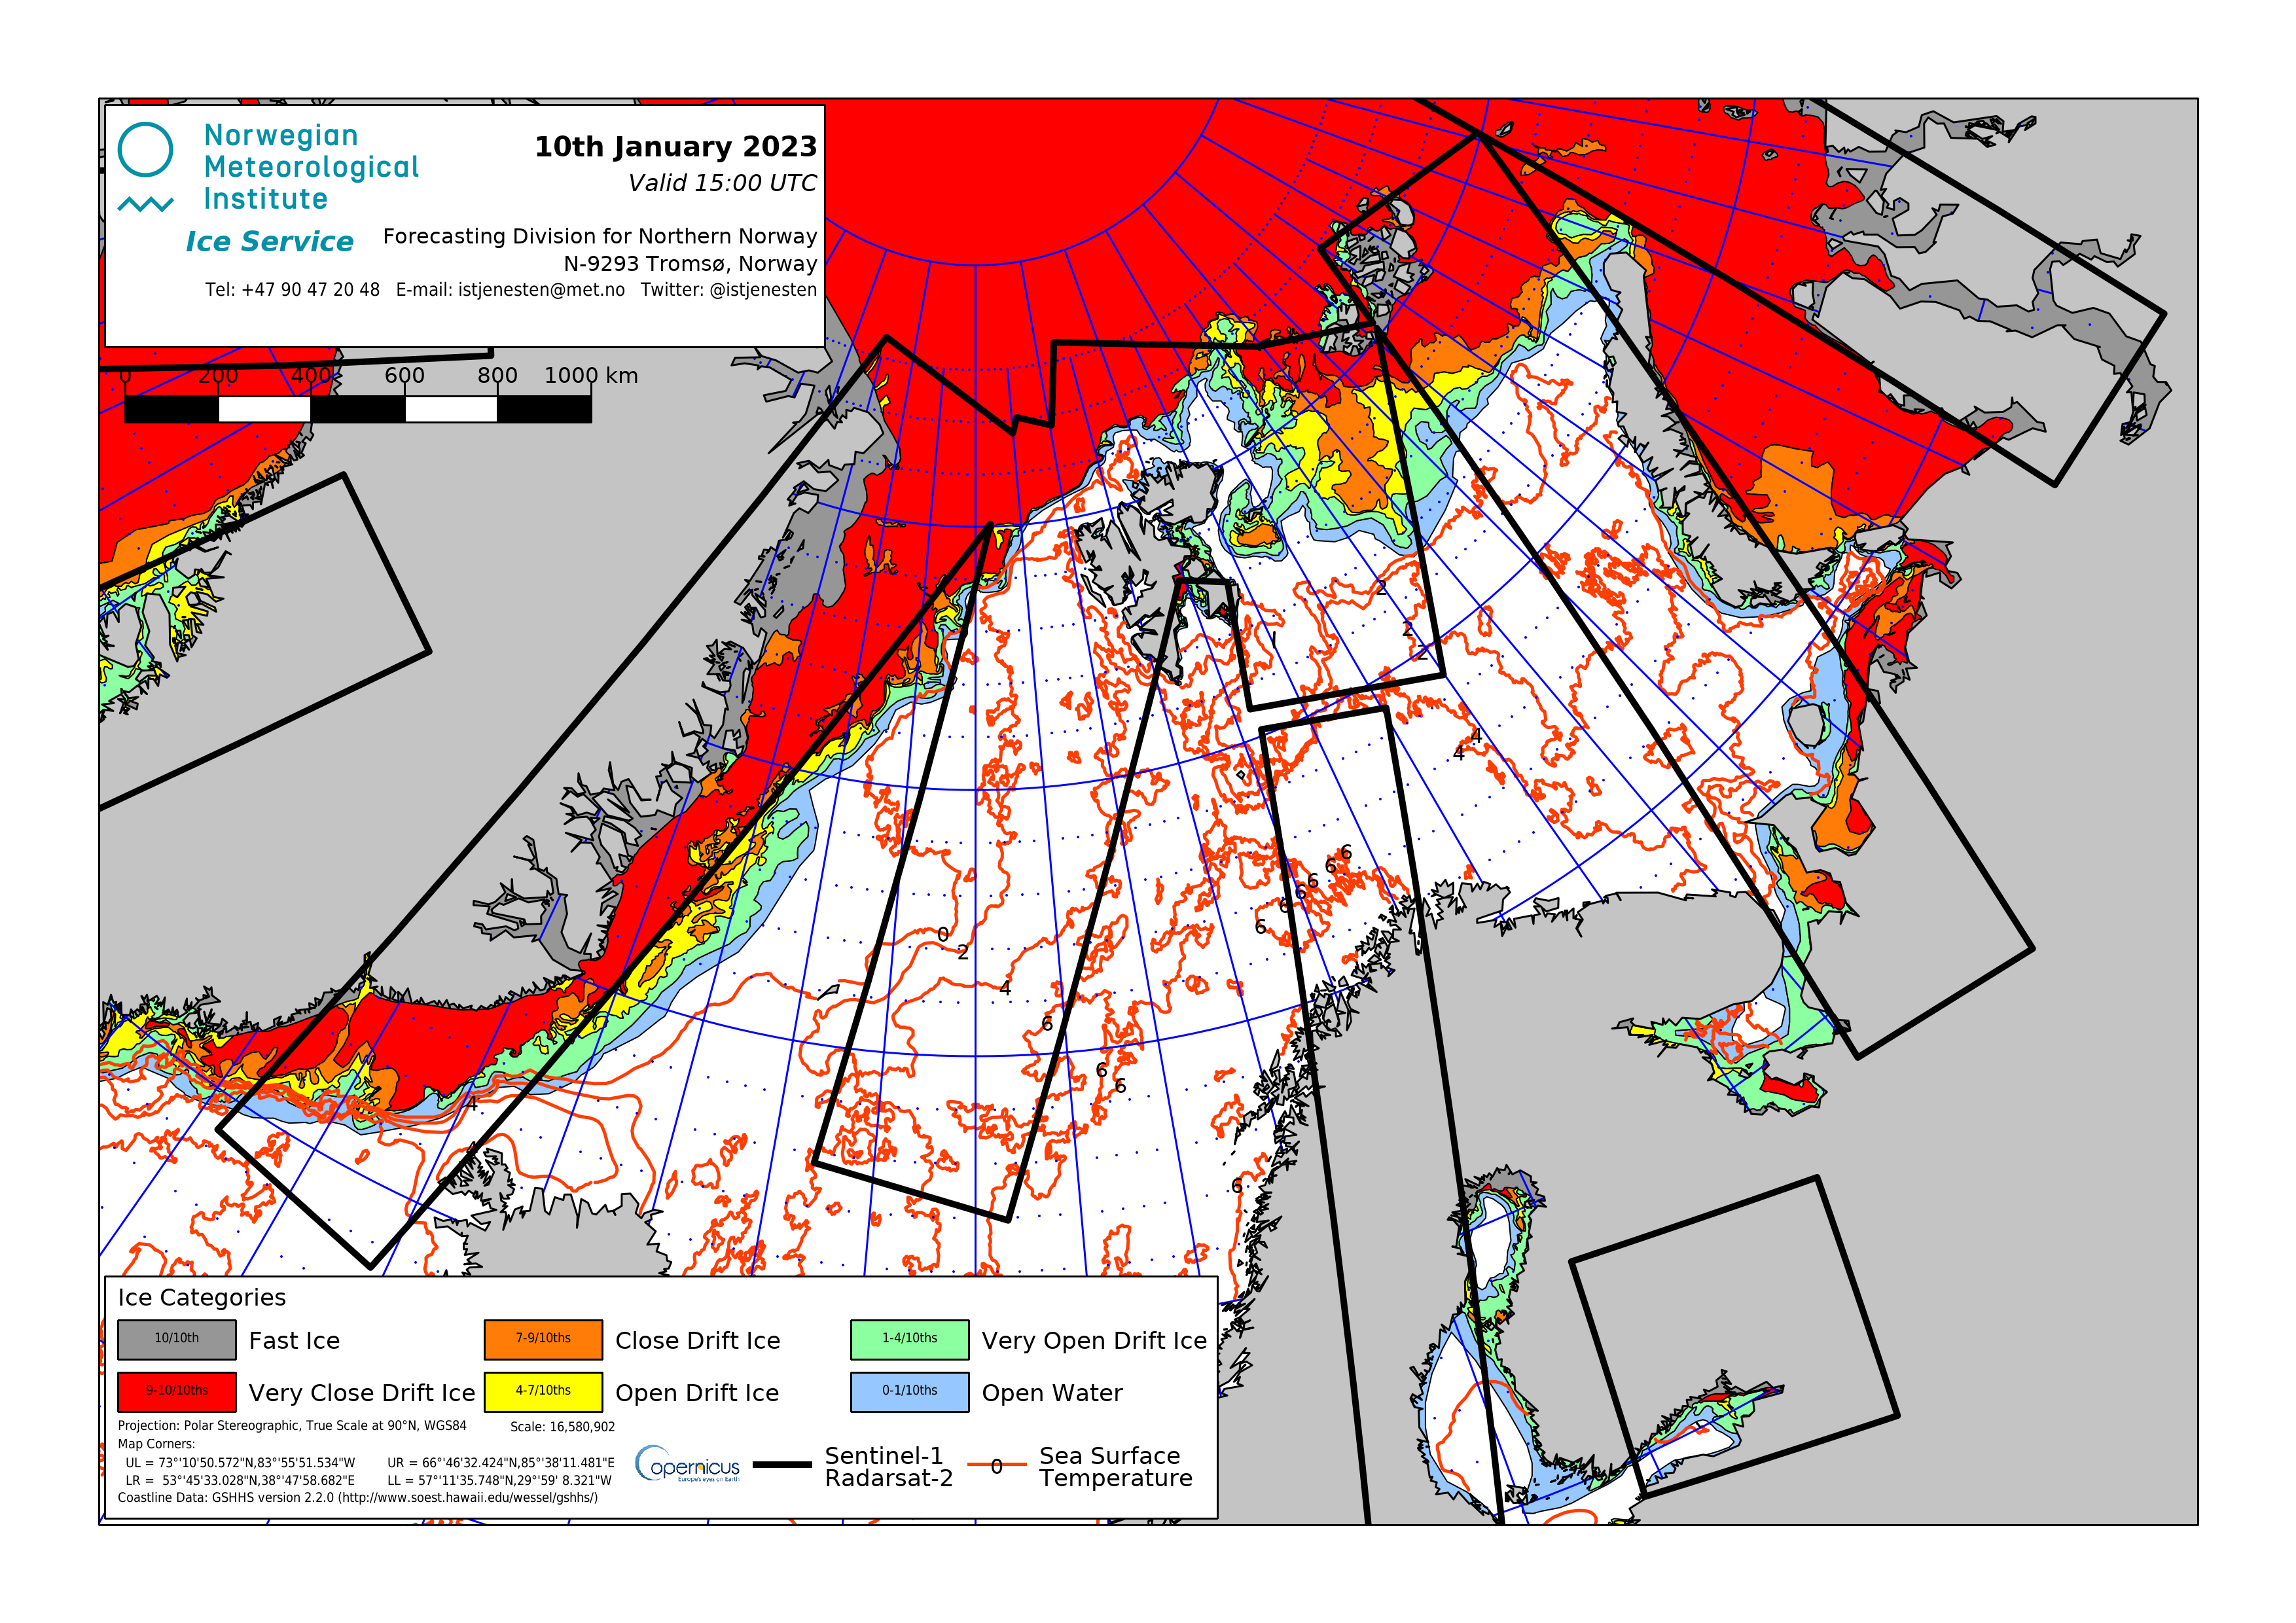
\includegraphics[width=\textwidth]{general_latest}
\end{figure}


\subsubsection{Osi-Saf}
Two different Sea Ice Concentration products are used from OSI-SAF. OSI-SAF SSMIS is an operational product delivering daily sea ice concentration on the northern (and southern) hemisphere. Whereas OSi-SAF Climate Data Record version 2 \cite{Soerensen2021} deliver sea ice climatology beginning in 1979 \cite{Lavergne2019}. The operational product will be used as a predictor for the model, whereas the climatology will be used only for validation purposes.

OSI-SAF SSMIS is a passive microwave product derived from the Special Sensor Microwave Imager and Sounder (SSMIS). To convert brightness temperature to estimated sea ice concentration, a hybrid approach combining the Bootstrap algorithm \cite{Comiso1997} and the Bristol algorithm \cite{Smith1996} where the prior is used over open water and the latter used for ice concentrations above 40\% \cite{Soerensen2021}. The end product is on a 10km polar stereographic grid.

The operational OSI-SAF SSMIS data is used to compute a coarse resolution (with respect to the ice charts) linear sea ice trend in each grid cell, with a length of 3 to 7 days. The idea behind the computed trend is to encode multiple time-steps of sea ice concentration fields into a single 2d-array, in line with the lack of temporal awareness of network \todo{not mentioned} as well as the limited available memory for training the model due to the high resolution data which limits the number of predictors. Furthermore, the ice concentration trend is computed from a separate sea ice product than the ice chart, with the intent to supply the model with correlated but not overlapping information, as the current day ice chart is already used as a predictor. The coarser resolution also contribute to the OSI-SAF trend serving as complementary information to the ice charts, as the coarse resolution make the trend less resolvent of the local variability which is seen in the ice charts. As such, the trend serves as a indicator of where the sea ice growth is occurring.

The temporal length used when deriving trend will have an impact as to how accurate the computed trend reflects the current growth and retreat zones, especially with regards to the volatile position of the ice edge on a daily timescale but also due to the seasonal variability of the ice area \cite{Holand2016}. Hence, a too large lookbehind would cause a decorrelation between the current sea ice concentration and computed trend. On the other hand, the motivation behind computing the trend is that there exist a large and positive autocorrelation for sea ice concentration on a short time-range. 


\subsubsection{AMSR2}
SIC from the AMSR2 sensor on a 6.25 km grid resolution retrieved using the ASI algorithm \cite{Spreen2008}. 


\subsection{Forecasting systems}
 
\subsubsection{AROME Arctic}
A deep neural network can increase the skill of its predicitions by using correlated variables which provide additional information of the current state of Sea Ice. \todo{Dette må enten refreres til bakover i oppgaven eller siteres} For example, near surface winds influence the sea ice drift speed \cite{Spreen2011}, with the sea ice drift speed being inverse proportional to the sea ice concentration \cite{Yu2020}. Moreover, two meter temperature can also impact the growth of sea ice. AROME Arctic is a non-hydrostatic, convection resolving high-resolution weather forecasting system which covers the European Arctic \cite{Mueller2017}.




\subsubsection{NeXtSIM}
The NeXtSIM-f forecasting system uses a standalone sea ice model (NeXtSIM), and is not coupled with an ocean model \cite{Williams2021}. Furthermore, NeXtSIM differentiates itself from comparative physical sea ice models as it does not apply a rheology based on the Viscous-Plastic scheme. Note that the rheology of a sea ice model refers to how the model relates ice deformation and ice thickness with the internal stresses in the ice \cite{Hibler1979}. internal stress. Instead, NeXtSIM applies a brittle sea ice rheology, specifically the Maxwell elasto-brittle rheology which treats the sea ice as a brittle material rather than a viscous fluid \cite{Dansereau2016}.


\subsubsection{Barents-2.5}
Barents-2.5, (hereby Barents) is an in-development operational coupled ocean and sea ice forecasting model at MET Norway \cite{Roehrs2022}. The model has been in operation since September 2021. Barents poses the same resolution and projection as AA, i.e. Lambert Conformal Conic with a 2.5km resolution \cite{Roehrs2022,Mueller2017}. Furthermore, Barents also forecast with a lead time up to 66 hours, which is the same as AROME Arctic. Since Barents covers the same spatial domain as the deep learning system and forecast with a lead time close to three days, its predicted sea ice concentration will be used for validation purposes.

The sea ice model used in Barents is the Los Alamos sea ice model (CICE) version 5.1, which uses an Elastic Viscous Plastic sea ice Rheology \cite{Hunke2015}. Thus, the CICE model represents sea ice as a viscous fluid which creeps slowly given small stresses and deforms plastically under large stress. It is also noted that the elastic behavior was introduced to benefit the numerical aspects of the model, and can be considered unrealistic from a physical point of view \cite{Hunke1997}.

Barents includes an Ensemble Prediction System with 6 members executed for each of the four model runs situated at (00, 06, 12 and 18) \cite{Roehrs2022}. As part its forcing routine, Barents performs non-homogenous atmospheric forcing of its ensemble members, with one member of each ensemble being forced with AA while the rest of the members is forces using atmospheric data from ECMWF. As such, the member forced with AA seem to perform best with regards to ocean currents, but the atmospheric forcing's impact on SIC performance is unknown at the time of writing (Johannes Röhrs, 2022, pers. commun.). However, there is generally little spread within one ensemble with regards to sea ice \cite{Roehrs2022}.

The data assimilation scheme applied for Barents is a Deterministic Ensemble Kalman filter, which solves for the analysis though with a background error covariance matrix estimated as the variance of the ensemble of background members \cite{Roehrs2022}. Furthermore, it has been expressed by the developers of Barents that the model performance was unsatisfactory up until May / June 2022 due to spin up time of the data assimilation system (Johannes Röhrs, 2022, pers. commun.). This coincides with the formulation of the Ensemble Kalman filter as a Monte Carlo formulation of the Kalman filter \cite{Sakov2008}. Hence, it is expected that the data assimilation scheme used in Barents improves over time, resulting in a higher confidence in more recent predictions made by the system.







% Local bibliography
\biblio

\end{document}